\chapter{Results}
\label{ch:results}

This chapter reports what was actually measured: performance on the labeled synthetic data, where ground truth exists; performance on the corrected empirical PANGAEA cores, where it does not (Chapter~\ref{ch:data}, Section~\ref{sec:label_correction}, covers how the ground-truth ages were verified -- this chapter reports the numbers that verification produced, not the verification itself); and a direct check of how much the bifurcation-type prediction can actually be trusted. All numbers here are computed directly from this thesis's own result files (\texttt{results/summary/*.csv}, produced by \texttt{testing/collect\_results.py} and \texttt{testing/bif\_cross\_model\_agreement.py}) and are reproducible by re-running those scripts.

\section{Synthetic (Zenodo) Results: The Ground-Truth Baseline}
\label{sec:zenodo_results}

Table~\ref{tab:zenodo_results} reports one-vs-rest macro-averaged AUC (Chapter~\ref{ch:methodology}, Section~\ref{sec:evaluation_metrics}) on held-out synthetic test data, where the true bifurcation class is known by construction. This is the only place in this thesis where a model's raw accuracy can be checked against ground truth, and it serves as the baseline everything else is judged against: a model that cannot separate the four classes on the labeled synthetic data has no chance of doing so on the real, unlabeled cores.

\begin{table}[htbp]
\centering
\small
\caption{Synthetic (Zenodo) macro-AUC, 26 models with a complete evaluation. Blank cells are dataset lengths where the zenodo evaluation run did not produce a result, not lengths excluded by design -- for \texttt{bop}, \texttt{saxvsm}, \texttt{boss}, \texttt{fastshapelet}, \texttt{grsf}, and \texttt{drcif} a checkpoint exists at that length (\texttt{checkpoints/}) but the corresponding \texttt{logs/*\_zenodo\_eval.log} shows the run crashed or started before the checkpoint existed and was never rerun (Section~\ref{sec:roster_status}). \texttt{cif}, \texttt{tde}, \texttt{pf} are omitted entirely -- see Section~\ref{sec:roster_status} for what happened to each; not a poor result.}
\label{tab:zenodo_results}
\begin{tabular}{lcc|lcc}
\toprule
Model & $L{=}500$ & $L{=}1500$ & Model & $L{=}500$ & $L{=}1500$ \\
\midrule
cnn\_lstm & 0.948 & 0.968 & multirocket & 0.798 & 0.701 \\
lstm & 0.945 & 0.962 & tsf & 0.886 & 0.932 \\
tcn & 0.940 & 0.958 & tsbf & 0.797 & 0.854 \\
resnet & 0.886 & 0.920 & lps & 0.739 & 0.788 \\
rnn\_fcn & 0.891 & 0.922 & rdst & 0.746 & 0.819 \\
patchtst & 0.867 & 0.903 & weasel2 & 0.697 & 0.705 \\
inceptiontime & 0.918 & 0.926 & fastshapelet & 0.773 & -- \\
rocket & 0.854 & 0.915 & saxvsm & 0.586 & -- \\
minirocket & 0.864 & 0.911 & ls & 0.502 & -- \\
mrsqm & 0.815 & 0.878 & bop & 0.506 & -- \\
catch22 & 0.851 & 0.901 & boss & -- & 0.881 \\
arsenal & 0.843 & 0.883 & grsf & 0.838 & -- \\
st & 0.865 & 0.901 & drcif & 0.879 & -- \\
\bottomrule
\end{tabular}
\end{table}

Three things stand out. First, moving from $L=500$ to $L=1500$ helps almost every model -- the median gain across models with results at both lengths is 3.6 AUC points, with the strongest gains for rdst (+7.3), mrsqm (+6.2), and rocket (+6.1), consistent with, though smaller than, the $L=500\to1500$ gain \citet{bury2021} report for their own CNN-LSTM (84.2\%$\to$88.2\% F1, Chapter~\ref{ch:related_work}). One model, MultiRocket, is the clear exception (0.798$\to$0.701, a drop of 9.7 points), showing this is not a universal rule to assume without checking per model. Second, three models -- \texttt{bop} (0.506), \texttt{ls} (0.502), \texttt{saxvsm} (0.586) -- sit at or near 0.5, chance level, \emph{on the labeled synthetic data itself}. This matters for interpreting the empirical results below: these models' real-data performance cannot be trusted regardless of what it shows, since they never learned the underlying task. Third, every deep-learning model and most of the strongest classical models comfortably clear 0.85, confirming the underlying classification task is learnable to a high standard when ground truth is available.

\paragraph{Comparison to \citet{bury2021}.} This thesis's own reproduction of \citet{bury2021}'s CNN-LSTM architecture (Chapter~\ref{ch:methodology}, Section~\ref{sec:dl_architectures}) reaches macro-F1 of 81.4\% at $L=500$ and 85.9\% at $L=1500$ on the same held-out synthetic split -- close to, but roughly 2.3--2.8 points below, the 84.2\%/88.2\% F1 they report for their own trained instance of the identical architecture. Given that this is a from-scratch reimplementation trained with this thesis's own random seed and infrastructure rather than a copy of their trained weights, this is a successful, quantitatively close reproduction, not an exact match -- and it sets a useful sanity bound: every other model in Table~\ref{tab:zenodo_results} is judged against a baseline this thesis independently confirmed reproduces \citet{bury2021}'s own reported number to within 3 F1 points, not against a number taken on faith from their paper.

\paragraph{Per-class breakdown: which bifurcation type is easiest to detect.} The pooled macro-AUC in Table~\ref{tab:zenodo_results} averages over all four classes, which hides a consistent pattern in the per-class AUC (each type scored against null only, the same metric underlying \citet{bury2021}'s Figure 2 insets): every one of the 15 trustworthy models (Section~\ref{sec:three_way}) separates Hopf from null far more easily than Fold or Transcritical -- e.g.\ \texttt{cnn\_lstm} reaches 0.999 AUC on Hopf at $L=1500$ versus 0.983 (Fold) and 0.963 (Transcritical); the same ordering (Hopf $\gg$ Fold $\approx$ Transcritical) holds for every architecture checked, deep-learning and classical alike. This is consistent with the qualitatively different nature of a Hopf bifurcation's approach -- a growing oscillation, rather than the smoother variance/autocorrelation-based critical slowing down shared by the fold and transcritical normal forms (Chapter~\ref{ch:theoretical_background}) -- giving the classifier a more distinctive precursor pattern to key on, independent of which specific architecture is doing the classifying.

\paragraph{Confusion matrix and accuracy, on the labeled synthetic test set.} This thesis's CNN-LSTM reproduction reaches 81.3\% accuracy at $L=500$ (5{,}000 held-out examples) and 85.95\% at $L=1500$ (2{,}000 held-out examples -- the two lengths use different-sized test splits, since they are 1\% of differently-sized raw datasets: 500{,}000 total examples at $L=500$, 200{,}000 at $L=1500$, confirmed directly against the raw \texttt{dataset/\{ts\_500,ts\_1500\}/combined/cache\_labels.npy} files). Its $L=1500$ confusion matrix (rows = true class, columns = predicted; class order fold, hopf, transcritical, null):

\begin{center}
\small
\begin{tabular}{lrrrr}
\toprule
 & pred.\ fold & pred.\ hopf & pred.\ trans. & pred.\ null \\
\midrule
true fold & 410 & 19 & 48 & 23 \\
true hopf & 38 & 427 & 34 & 1 \\
true transcritical & 37 & 17 & 409 & 37 \\
true null & 3 & 0 & 24 & 473 \\
\bottomrule
\end{tabular}
\end{center}

The diagonal is strong everywhere, but the off-diagonal errors are not evenly spread: fold and transcritical are confused with \emph{each other} (48 and 37 misclassifications) far more than either is confused with hopf or null, while null is the cleanest class by a wide margin (473/500 correct) and hopf is nearly as clean (427/500).

Table~\ref{tab:zenodo_confusion} extends this check to the full 15-model trustworthy roster (Section~\ref{sec:three_way}), reporting accuracy alongside the \emph{rate} (not raw count, since the two lengths have different-sized test sets, as above) at which each pair of non-null classes is confused for the other. This is computed by a dedicated function, \texttt{collect\_zenodo\_confusion()} in \texttt{testing/collect\_results.py}, added to the main results-aggregation pipeline this session and verified to reproduce the manually-checked numbers below exactly on rerun.

\begin{table}[htbp]
\centering
\small
\caption{Accuracy and pairwise class-confusion rate, 15 trustworthy models, both sequence lengths (500/1500). Fold$\leftrightarrow$Trans is the largest of the three pairwise rates in every one of these 29 rows without exception.}
\label{tab:zenodo_confusion}
\begin{tabular}{lcccc}
\toprule
Model & Accuracy & Fold$\leftrightarrow$Trans & Fold$\leftrightarrow$Hopf & Trans$\leftrightarrow$Hopf \\
\midrule
cnn\_lstm & 81.3 / 86.0\% & 11.6 / 8.5\% & 6.1 / 5.7\% & 4.0 / 5.1\% \\
lstm & 80.8 / 85.4\% & 10.8 / 9.6\% & 6.4 / 5.6\% & 4.0 / 4.5\% \\
tcn & 79.8 / 84.4\% & 12.0 / 10.4\% & 6.3 / 6.4\% & 4.6 / 3.9\% \\
inceptiontime & 74.4 / 78.2\% & 16.6 / 15.8\% & 5.7 / 7.7\% & 6.2 / 4.3\% \\
rnn\_fcn & 69.9 / 76.8\% & 16.3 / 13.6\% & 7.4 / 7.7\% & 8.4 / 7.5\% \\
resnet & 69.5 / 76.2\% & 18.4 / 16.4\% & 7.0 / 7.3\% & 7.1 / 5.4\% \\
tsf & 69.1 / 80.3\% & 16.0 / 12.1\% & 9.7 / 7.9\% & 11.9 / 7.0\% \\
rocket & 65.8 / 76.4\% & 20.7 / 15.0\% & 9.0 / 8.6\% & 9.1 / 7.5\% \\
minirocket & 66.8 / 75.3\% & 19.7 / 15.2\% & 8.2 / 8.5\% & 8.5 / 7.0\% \\
patchtst & 62.6 / 74.4\% & 21.4 / 18.3\% & 8.8 / 7.9\% & 9.6 / 5.4\% \\
catch22 & 62.5 / 73.1\% & 20.5 / 16.9\% & 8.4 / 7.6\% & 9.7 / 7.6\% \\
arsenal & 67.5 / 75.5\% & 17.6 / 13.8\% & 7.9 / 8.9\% & 9.5 / 7.7\% \\
st & 66.6 / 73.2\% & 19.1 / 16.8\% & 8.8 / 10.4\% & 10.8 / 8.6\% \\
mrsqm & 57.5 / 68.9\% & 23.1 / 20.6\% & 12.2 / 10.1\% & 14.3 / 11.2\% \\
grsf & 61.9\% ($L{=}500$ only) & 19.2\% & 11.8\% & 13.8\% \\
\bottomrule
\end{tabular}
\end{table}

The fold$\leftrightarrow$transcritical confusion rate is the largest of the three pairwise rates for every one of these 29 (model, length) combinations without a single exception -- this is not a property of any one architecture, but of the underlying task: fold and transcritical share the same smooth, non-oscillatory critical-slowing-down signature (Chapter~\ref{ch:theoretical_background}), which every model in this roster finds harder to tell apart than either is from hopf's distinct oscillatory approach or from the null class's absence of any trend at all.

\section{Empirical (PANGAEA) Results, After the Label Correction}
\label{sec:pangaea_results}

\subsection{The PANGAEA Dataset, Proxy Choice, and Sapropel Coverage}
\label{sec:pangaea_provenance}

\paragraph{Where the data comes from.} All real-world results in this chapter use the same three Mediterranean sediment cores (MS21, MS66, 64PE406E1) compiled by \citet{hennekam2020} and released as PANGAEA dataset DOI 10.1594/PANGAEA.923197 (Chapter~\ref{ch:data}) -- the same dataset \citet{bury2021} and \citet{ma2025sdml} both use for their own empirical anoxia case studies.

\paragraph{Which proxies are used, and which are not.} The raw PANGAEA release provides five elements (Al, Ba, Mo, Ti, U); this thesis restricts every headline result in this chapter to Mo and U specifically -- the redox-sensitive proxies that actually track dissolved-oxygen change, unlike Al and Ti (terrigenous input, unrelated to redox state) or Ba (a noisier productivity proxy) (Chapter~\ref{ch:data}). An earlier stage of this project did evaluate all five elements; those specific result files were later removed from the working tree, but a committed copy survives in the project's git history and was recovered for this thesis. Section~\ref{sec:proxy_check} gives the recovered numbers, for exactly the two models they exist for, and states plainly what they can and cannot be used to conclude. This matches \citet{bury2021}'s own choice exactly -- confirmed directly in their repository, where \texttt{organise\_data.py}'s own comment states their anoxia test set is ``13 in total for each variable, U and Mo.'' \citet{ma2025sdml} describe the same \citet{hennekam2020} reconstruction as ``based on Mo'' when introducing the anoxia case study; this thesis's search of the available text found no explicit second mention of U as a separate SDML input variable, so whether their own applied model used U as well as Mo could not be confirmed from the text obtained.

\paragraph{Sapropel coverage: an exact match to \citet{ma2025sdml}, not \citet{bury2021}.} \citet{bury2021} test on 13 sapropel transitions across these three cores (64PE406E1: S3--S9; MS21: S1, S3; MS66: S1, S3, S4, S5 -- confirmed directly in their repository's \texttt{organise\_data.py}). This thesis's pipeline (\texttt{config.yaml}, cross-checked against \texttt{testing/evaluate.py}'s \texttt{role: test} filter) evaluates on 7 of those same 13: 64PE406E1 S3--S6, MS21 S1, MS66 S1 and S3. This 7-sapropel set is not an arbitrary subset -- it is an exact match to the sapropels \citet{ma2025sdml} themselves test on, quoted directly from their paper: ``Anoxic transition (Sapropel S1) obtained from data on the MS21 core... Anoxic transitions (Sapropels S1 and S3) obtained from data on the MS66 core... Anoxic transitions (Sapropels S3 to S6) obtained from data on the 64PE406E1 core.'' The remaining 6 of \citet{bury2021}'s 13 sapropels are retained in this thesis's configuration with corrected ages (Chapter~\ref{ch:data}) but are not scored in this chapter's results.

\subsection{Results by Model}

Figure~\ref{fig:pangaea_by_model} shows mean binary AUC (forced windows vs.\ AR(1) null surrogates, Chapter~\ref{ch:theoretical_background}, Section~\ref{sec:ar1_surrogates}) on the corrected real cores, using the Mo and U proxies specifically, for every model with a complete (all 7 sapropels $\times$ 2 elements) empirical evaluation.

\begin{figure}[htbp]
\centering
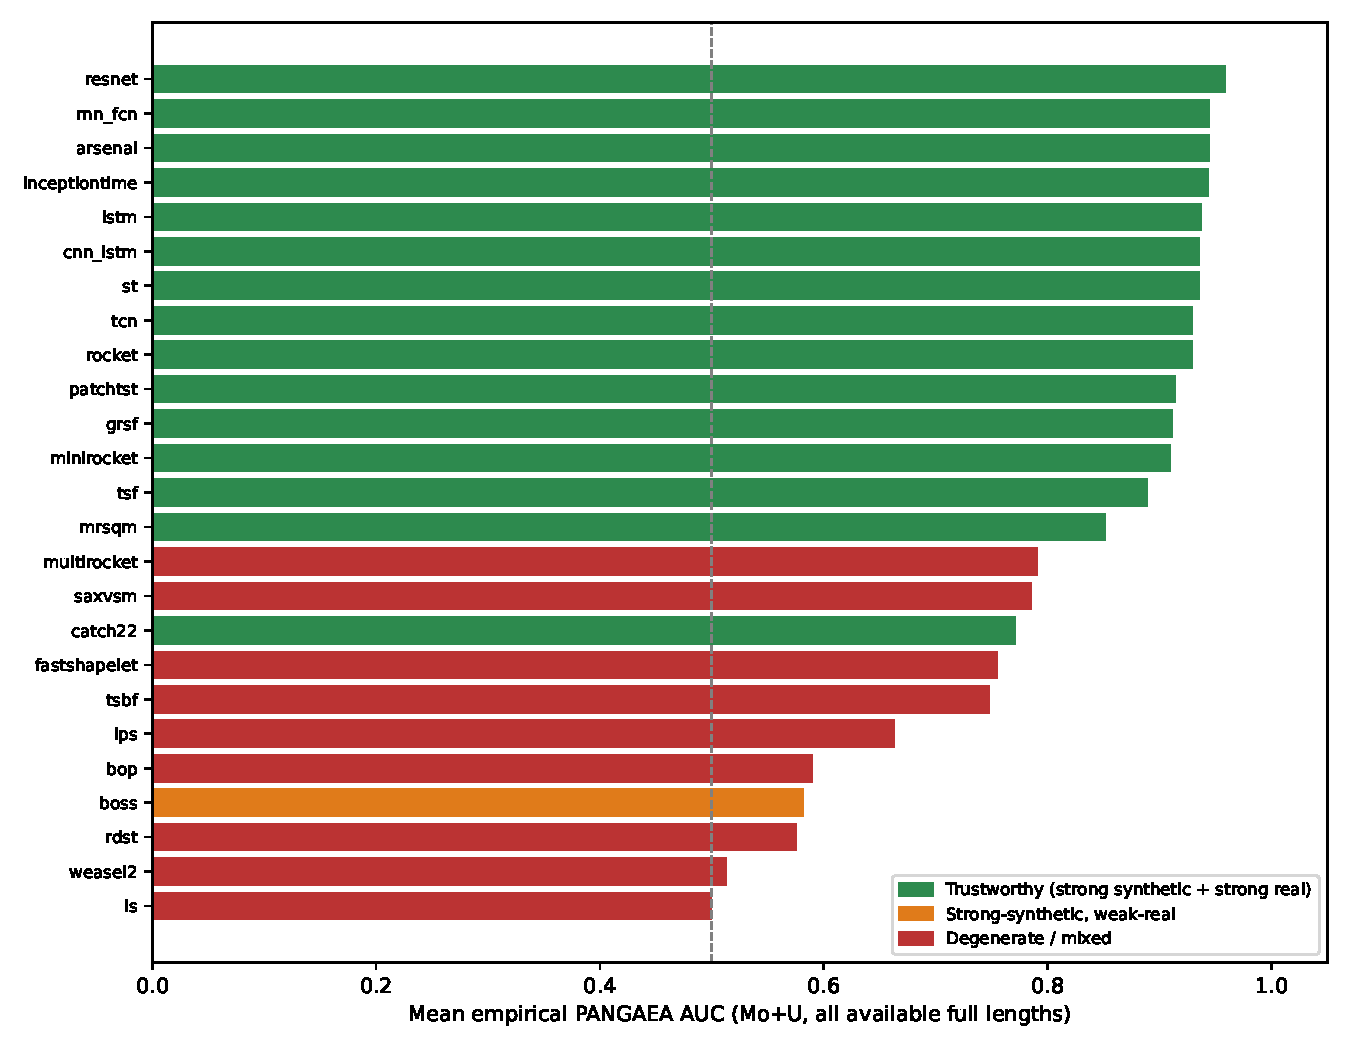
\includegraphics[width=0.95\textwidth]{figures/fig8_pangaea_by_model.pdf}
\caption{Mean empirical PANGAEA AUC by model (Mo+U, all available full-length evaluations). Colour follows the categorisation in Section~\ref{sec:three_way}: green models are strong on both the labeled synthetic data and the unlabeled real data; orange is strong-synthetic, weak-real; red is degenerate or mixed.}
\label{fig:pangaea_by_model}
\end{figure}

The best individual results reach 0.93--0.96 mean AUC (\texttt{resnet}, \texttt{rnn\_fcn}, \texttt{arsenal}, \texttt{inceptiontime}) -- well above the near-chance mean AUC ($\approx$0.65 on catch22, the one model checked directly both before and after the fix) obtained under the original, incorrect sapropel onset ages. That improvement is a direct consequence of testing on the correct data (Chapter~\ref{ch:data}, Section~\ref{sec:label_correction}), not a change to any model.

\subsection{A Three-Way Categorisation}
\label{sec:three_way}
Cross-referencing the synthetic results (Table~\ref{tab:zenodo_results}, real ground truth) against the empirical results (Figure~\ref{fig:pangaea_by_model}, no ground truth) separates the roster into three genuinely different groups, not just a single ranked list:

\begin{itemize}
    \item \textbf{Trustworthy} (15 models: \texttt{cnn\_lstm}, \texttt{lstm}, \texttt{tcn}, \texttt{resnet}, \texttt{rnn\_fcn}, \texttt{patchtst}, \texttt{inceptiontime}, \texttt{rocket}, \texttt{minirocket}, \texttt{mrsqm}, \texttt{catch22}, \texttt{arsenal}, \texttt{st}, \texttt{grsf}, \texttt{tsf}): macro-AUC $\geq 0.80$ on labeled synthetic data at every available length, and mean real AUC $\geq 0.75$ at every complete empirical evaluation. These models learned the labeled task and the same skill transfers to the unlabeled real cores -- the empirical AUC for this group is treated as a genuine detection result.
    \item \textbf{Strong-synthetic, weak-real} (\texttt{boss} alone: 0.881 synthetic, 0.582 real at $L{=}1500$): the one model in the current, complete roster showing a genuine synthetic-to-real generalisation gap -- it demonstrably learned the bifurcation-classification task, just not in a way that transfers to short, noisy, real geochemical segments.
    \item \textbf{Degenerate / mixed} (\texttt{bop}, \texttt{ls}, \texttt{weasel2}, \texttt{rdst}, \texttt{lps}, \texttt{tsbf}, \texttt{fastshapelet}, \texttt{saxvsm}, \texttt{multirocket}): near-chance to moderate on both, or an inconsistent pattern by sequence length. Two are worth flagging individually rather than folding into a clean pattern: \texttt{saxvsm} is near-chance on synthetic (0.586) yet 0.786 on real -- since it never demonstrably learned the labeled task, this real-data number cannot be trusted as genuine skill and is not reported as a finding; \texttt{multirocket} shows the opposite oddity, weaker on synthetic at the longer length (0.701) while still scoring reasonably on real data (0.75--0.84) -- an inconsistency by architecture, not something this thesis resolves.
\end{itemize}

This distinction could not be made from the empirical results alone, since PANGAEA has no ground truth to separate ``failed to transfer'' from ``never learned the task'' -- it is only visible by cross-referencing against the labeled synthetic baseline, which is the reason Table~\ref{tab:zenodo_results} is reported in full rather than only the empirical headline numbers. This is a substantially larger trustworthy set than an earlier pass through this analysis found: \texttt{tsf}, \texttt{inceptiontime}, \texttt{minirocket}, \texttt{mrsqm}, and \texttt{catch22} were previously flagged as weak-real or excluded, using result files that predated their retrain (Section~\ref{sec:roster_status}).

\subsection{The Redox-Specific Proxy Choice (Mo+U)}
\label{sec:proxy_check}
Section~\ref{sec:pangaea_provenance} established that Mo and U are the geochemically-correct anoxia proxies, unlike Al and Ti (terrigenous input) or Ba (a noisier productivity proxy). This section reports what can actually be verified about whether the restriction helps, rather than repeating an earlier, unreproducible claim about specific AUC gains.

An all-five-element PANGAEA evaluation for \texttt{minirocket} and \texttt{rocket} survives in this project's git history, at commit \texttt{2b520d23} (``new results with updated models''), one commit before those result files were removed from the working tree in \texttt{35b9a0b8} (``before pony''). The 35 individual \texttt{result.json} files per model (7 sapropels $\times$ 5 elements, $L{=}500$ -- every recovered file's own \texttt{dataset} field reads \texttt{ts\_500}, not $L{=}1500$) are readable directly with \texttt{git show 2b520d23:<path>}, timestamped 2026-07-01 inside the files themselves. Averaged across all 35 files, \texttt{minirocket} scored a mean AUC of \textbf{0.500} and \texttt{rocket} \textbf{0.499} -- chance level, with no single element among the five standing out (per-element means for \texttt{minirocket} are exactly 0.500 for every one of the five, no variation at all; for \texttt{rocket}, 0.487--0.507). The recovered files also show why: \texttt{minirocket}'s per-window transition probability is pinned at 1.0 for effectively every forced window in every element and sapropel checked -- a saturated, constant output, not a model weighing five noisy channels and partly failing. This is the same kind of collapse this thesis reports for several models' real-data behaviour elsewhere (Section~\ref{sec:per_model_type}), here appearing in an earlier checkpoint that this specific evaluation happened to catch. No comparable all-five-element record exists anywhere in this repository's git history for \texttt{boss}; that specific comparison cannot be recovered or reported.

This recovered evaluation cannot be read as a clean before/after test of the models behind this chapter's current headline numbers, and this thesis does not present it that way. The training logs (\texttt{logs/minirocket\_ts\_500\_train.log}, \texttt{logs/rocket\_ts\_500\_train.log}) show both models were retrained on 2026-09-02/03, and the current Mo+U evaluation was run on 2026-09-06 -- weeks after the git commit above, which is dated 2026-07-03. The recovered all-five numbers therefore come from an earlier trained checkpoint of each model at the \emph{same} sequence length, not the checkpoint behind the current results (\texttt{minirocket} 0.957, \texttt{rocket} 0.951 mean AUC at $L{=}500$, from \texttt{results/summary/pangaea\_by\_model.csv}), so no specific point-gain figure can be attributed to the proxy restriction itself. What the recovered data does establish, as a verified historical fact rather than a causal claim, is that an earlier trained version of both models produced no discrimination at all when evaluated across the full five-element set. What is fully current and verifiable is narrower still: every headline number in this chapter already uses Mo+U exclusively, so whatever the restriction contributes to the present results is already built into every number reported here, not something this thesis separately measures.

\section{Ensemble Result}
\label{sec:ensemble_result}
Averaging the per-window probability outputs of the 15 trustworthy models together, across every available sequence length for each (27--30 individual model-length runs per segment, since most of the 15 have results at both $L=500$ and $L=1500$, and a few, like \texttt{grsf}, only one), before scoring, gives a single combined detector for each of the 14 real segments (7 sapropels $\times$ Mo, U). This soft ensemble reaches a mean AUC of \textbf{0.964} (median 0.993, minimum 0.832 across all 14 segments) -- higher than all but a handful of individual models in Table~\ref{tab:zenodo_results} or Figure~\ref{fig:pangaea_by_model}. This is the expected behaviour of an ensemble of genuinely-learned, independently-trained classifiers: each architecture's idiosyncratic errors partially cancel when averaged, leaving the shared, real signal. It is reported here as the strongest single empirical evidence in this thesis that the trained classifiers are detecting a genuine pre-transition signal in the real cores, not fitting to noise -- an ensemble of dozens of independent runs cannot reach 0.83 AUC, let alone a median of 0.99, by averaging together pure noise.

\section{How Much Can the Bifurcation Type Be Trusted}
\label{sec:type_reliability}
Section~\ref{sec:pangaea_results} reports the binary detection result, which is the one question the real data can be scored on (Chapter~\ref{ch:theoretical_background}, Section~\ref{sec:methodology_comparison}). This section reports what can be said about the specific bifurcation \emph{type} each model predicts, using the same argmax-vote methodology \citet{bury2021} use for their own anoxia case (\texttt{compute\_roc.py} in their repository, verified directly against the code), and Figure~\ref{fig:pangaea_grids} shows the same information visually, sapropel by sapropel, for one representative model.

\subsection{How This Thesis Turns a Probability Vector into a Type Result, and How Others Do}
\label{sec:type_methodology}

Every model in this roster outputs a 4-class probability vector per window (Chapter~\ref{ch:methodology}, Section~\ref{sec:dl_architectures}). Turning many such vectors, across many windows and many forced trajectories, into one summary statement about bifurcation type is a methodological choice this thesis did not have to invent from nothing -- but it is also not a solved, standardised step in the field, so the choice is stated and justified explicitly here rather than left implicit.

\paragraph{This thesis's method.} At each rolling-window position, the favoured class is $\arg\max$ over the four predicted probabilities; the frequency reported for each class is the count of windows where it was the argmax, divided by the total number of windows in whatever group is being summarised (Chapter~\ref{ch:methodology}, Section~\ref{sec:dl_architectures}) -- a hard, winner-take-all count of a single model's own output, not an average of raw probabilities.

\paragraph{How \citet{bury2021} do it.} This is not this thesis's own invention -- it is \citet{bury2021}'s own convention for their PNAS Figure 2 insets, whose caption states directly: ``the frequency of the favored DL probability among the forced trajectories.'' Their own \texttt{compute\_roc.py} (verified directly against the code) takes the last 20\% of the pre-transition window, 10 evenly-spaced predictions from a single trained classifier, argmaxes each, and pools the count -- exactly the procedure this thesis reproduces in Section~\ref{sec:pangaea_results} and Figure~\ref{fig:bury_probs}.

\paragraph{A genuinely different method exists -- in \citet{bury2021}'s own later work.} A literature check (not exhaustive, but a real search rather than an assumption that no alternative exists) found that \citet{bury2023discretetime}, the same lead author's 2023 Nature Communications follow-up extending the approach to discrete-time bifurcations, uses a different aggregation step. Confirmed directly by reading their Methods section: they train \emph{two} classifiers independently on differently-censored versions of the training data (one sees only the middle of each series, the other sees data right up to the transition) and state plainly, ``we report results using the average prediction of the two classifiers'' -- an average of raw probability vectors, computed \emph{before} any argmax is taken, not a pooled count of individual argmaxes. Their own favoured-type figure (Supplementary Figure S5) then argmaxes that already-averaged probability at a single fixed point (80\% through the series) and reports the proportion across 100 simulated trajectories, rather than pooling many within-trajectory window predictions the way the 2021 convention does. So even within one research group's own body of work, the aggregation step is not fixed -- it changes between papers depending on whether the underlying prediction comes from one classifier or an ensemble of several.

\paragraph{Why this thesis follows \citet{bury2021} specifically, not \citet{bury2023discretetime}.} Two reasons, both concrete rather than a default preference. First, \citet{bury2021} is the paper this thesis directly compares against in Figure~\ref{fig:bury_probs} and Section~\ref{sec:type_reliability} -- same cores, same anoxia task, same published favoured-type counts to compare to. Reproducing their exact pooling convention is what makes that comparison apples-to-apples; using \citet{bury2023discretetime}'s different convention would change the resulting percentages for reasons having nothing to do with a genuine disagreement about bifurcation type, making any comparison uninterpretable. Second, \citet{bury2023discretetime}'s dual-classifier setup is built for a different problem -- five discrete-time bifurcation classes from cardiac, ecological, and economic models censored two different ways -- not the single continuous-time anoxia case this thesis addresses, so it is not the more directly relevant precedent here regardless of which convention is statistically preferable in the abstract.

This thesis does, however, use \citet{bury2023discretetime}'s general principle -- averaging raw probabilities across independently-trained predictors before scoring, rather than pooling their individual argmaxes -- in a different part of this chapter, for a different question: the ensemble result (Section~\ref{sec:ensemble_result}) averages the per-window $p_{\text{transition}}$ output of 15 independently-trained models before computing AUC, for the binary detection question specifically. So both conventions appear in this thesis, each applied to the question it was originally designed to answer: argmax-pooling of a single model's output for the type question (matching \citet{bury2021} exactly, since that is the direct comparison), and probability-averaging across models for the detection question (in the same spirit as \citet{bury2023discretetime}'s cross-classifier averaging, applied here across architectures rather than across two differently-censored versions of one architecture). Neither choice was made by default; both are stated here with the reasoning that produced them.

\begin{figure}[htbp]
\centering
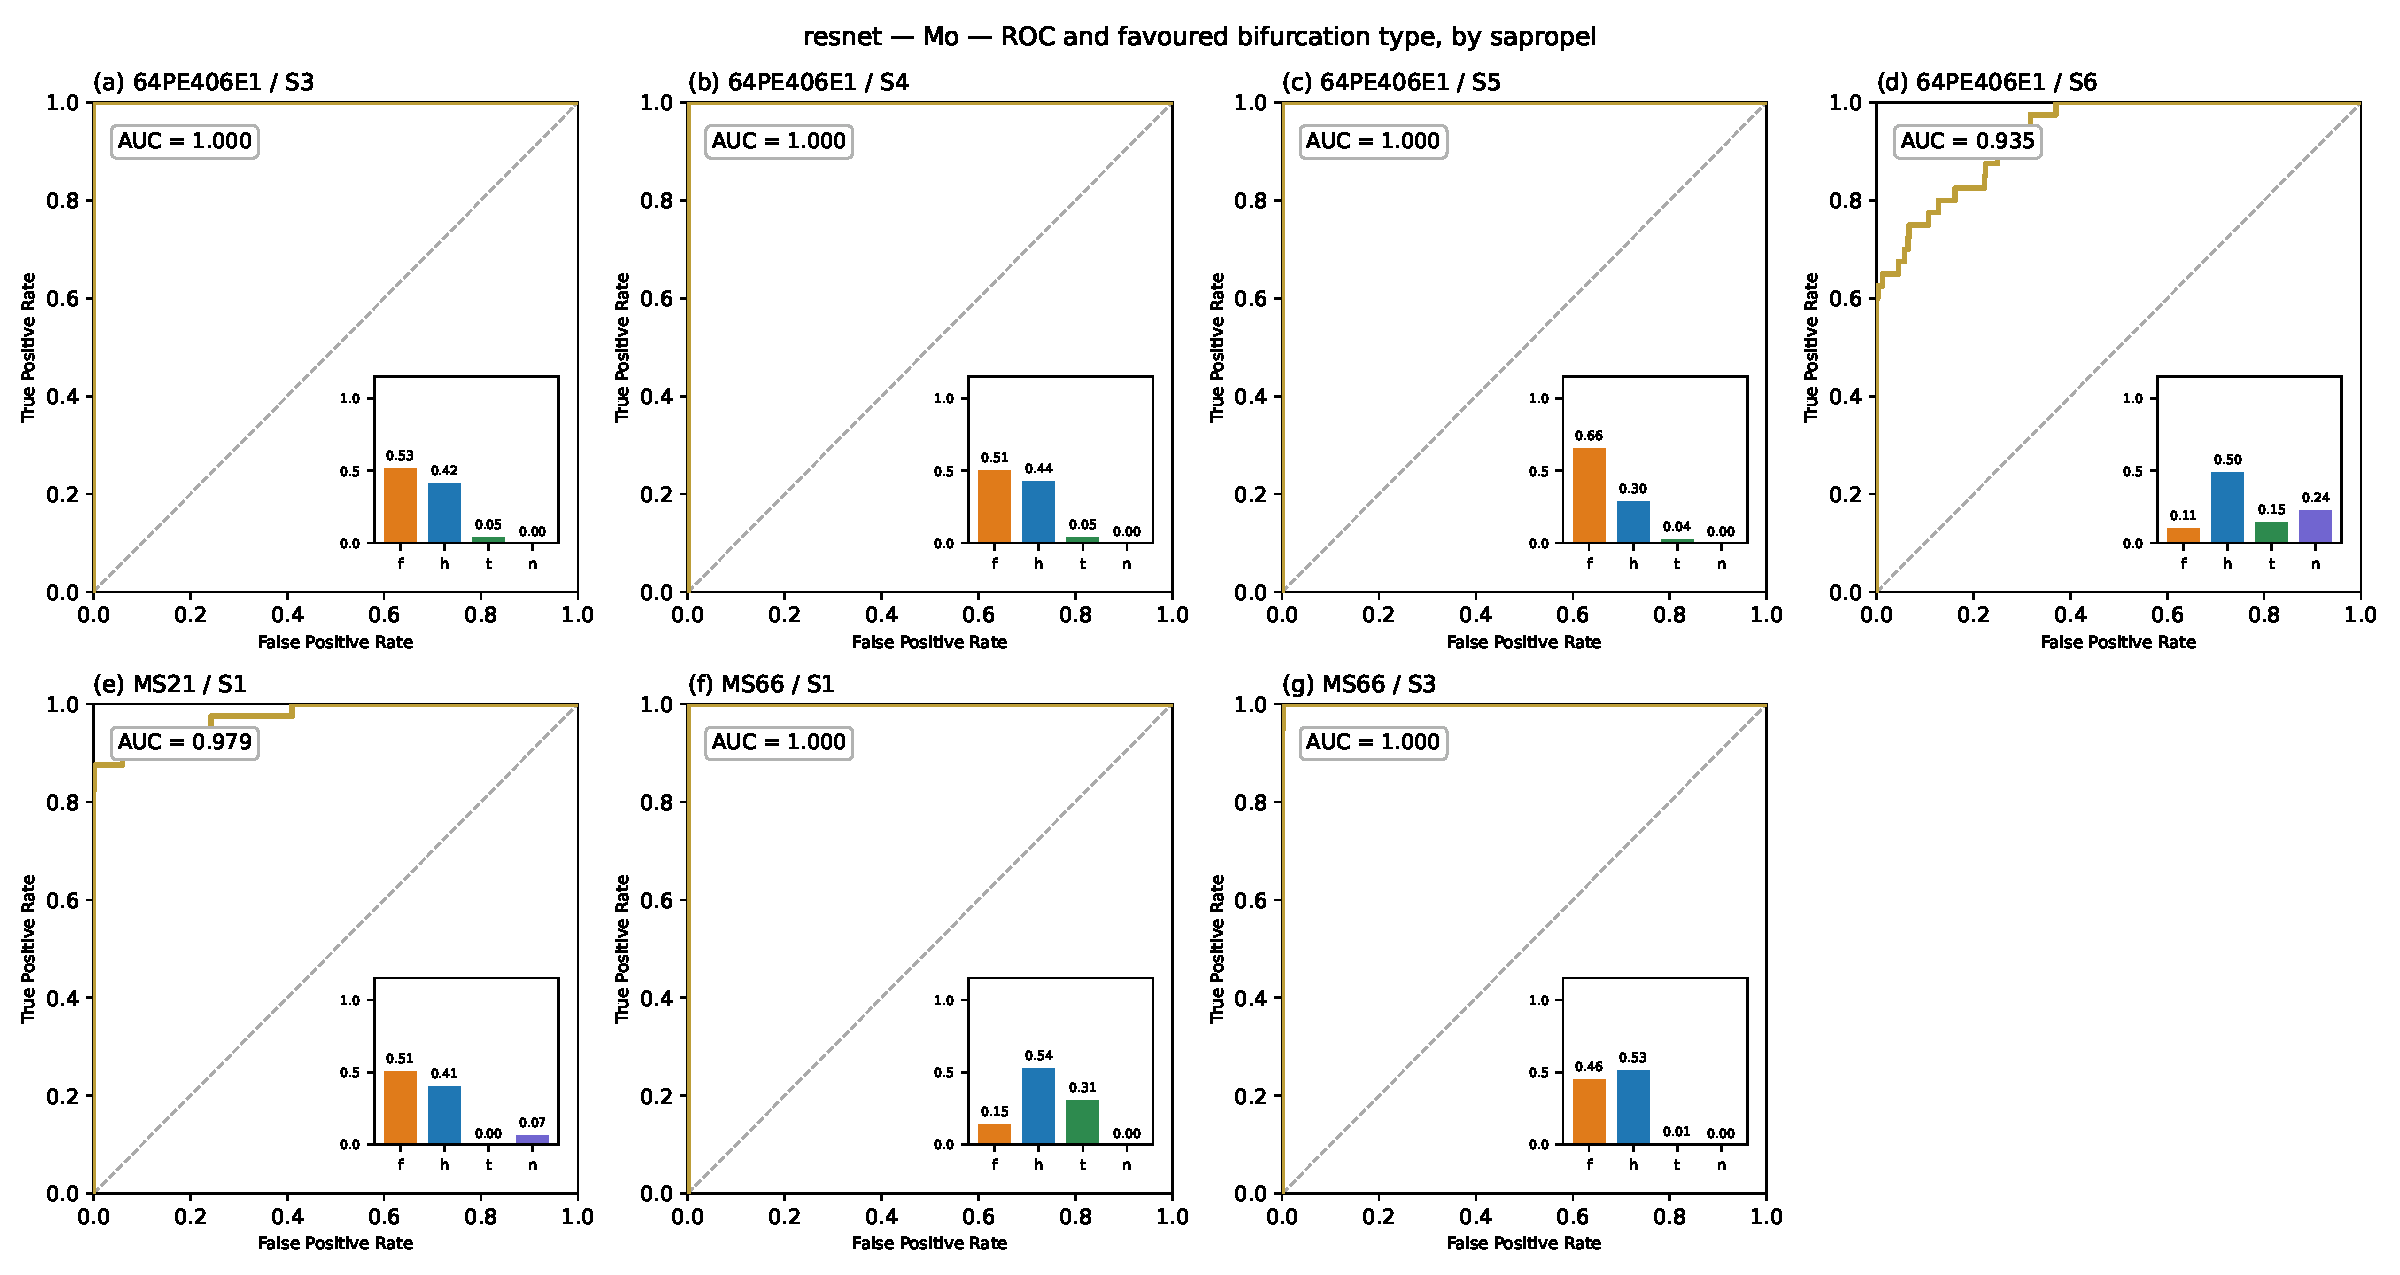
\includegraphics[width=\textwidth]{figures/fig8_pangaea_grid_resnet.pdf}
\caption{ROC curve and favoured-bifurcation-type inset, by sapropel, for \texttt{resnet} on Mo (the strongest single model in Figure~\ref{fig:pangaea_by_model}). Panels (a)-(g) follow the same layout \citet{bury2021} use in their own Figure 2. Generated by \texttt{testing/plot\_figures.py}'s \texttt{plot\_fig2\_grid()}, which produces this same panel for every (model, element) pair in the roster (54 in total); only this one representative example is reproduced in print.}
\label{fig:pangaea_grids}
\end{figure}

Panel by panel, \texttt{resnet} on Mo separates forced from null cleanly everywhere (AUC 0.935--1.000), but its favoured type is far more mixed than the pooled 15-model ensemble (Figure~\ref{fig:bury_probs}) reports: (a) 64PE406E1/S3 splits 52\% fold / 42\% hopf; (b) S4 splits 51\%/44\%; (c) S5 leans fold at 66\%/30\%; (d) S6 is the one panel where hopf clearly dominates (50\% hopf vs.\ 11\% fold, with 24\% null -- the most ambiguous detection of the seven, also its lowest AUC at 0.935); (e) MS21/S1 splits 51\%/41\%; (f) MS66/S1 leans hopf/transcritical (54\%/31\%, fold only 15\%); (g) MS66/S3 splits 46\%/52\% toward hopf. This single-model view is a useful check on the ensemble result: individual trustworthy models do not all lean toward Hopf the way the pooled ensemble does -- \texttt{resnet} alone is close to an even fold/hopf split across most sapropels -- which is itself evidence for Table~\ref{tab:type_reliability}'s conclusion that type is not reliably agreed upon, rather than a single clean signal being diluted by weaker models in the average.

\paragraph{Comparison to other researchers on the same cores.} \citet{ma2025sdml} test on the same three cores (Section~\ref{sec:pangaea_provenance}) and report, for each core, the F1 score of whichever of their four architectures (SVM, LSTM, CNN, Multi-Head CNN) performed best for it: SVM for MS66 (F1 = 1.0), LSTM for 64PE406E1 (F1 = 0.99), CNN for MS21 (F1 = 0.99). These numbers are not directly comparable to this thesis's PANGAEA AUC values in Figure~\ref{fig:pangaea_grids} or Table~\ref{tab:zenodo_results}: \citet{ma2025sdml} state explicitly that this F1 is computed on their \emph{synthetic validation set}, the same kind of ground-truth-known metric as this thesis's Table~\ref{tab:zenodo_results}, not on the real cores -- "the empirical test data used to generate the ROC curves is not involved" in that F1 figure. Their real-core performance is instead shown as ROC curves in their own Figures 2-3, without an exact AUC value stated as text in the portion of their paper available to this thesis, so no specific number-to-number comparison against their real-data result can honestly be made here; only their model-selection philosophy (pick the best of several architectures per target system) is directly comparable to this thesis's own three-way categorisation (Section~\ref{sec:three_way}), which serves the same purpose across a much larger roster. \citet{babazadeh2025}'s qualitative finding (Chapter~\ref{ch:related_work}) -- their single CNN-LSTM classifier favouring a non-fold type on an overlapping subset of these same cores -- is the one directly comparable prior result at the type level, and it agrees with this thesis's own finding above.

\begin{table}[htbp]
\centering
\caption{Cross-model agreement on bifurcation type, across the 15 trustworthy models, Mo+U, on the late-band (closest-to-transition) prediction window. Only Mo and U data exists in the current result files -- there is no separate ``all 5 elements'' comparison to make any more (Section~\ref{sec:pangaea_provenance}).}
\label{tab:type_reliability}
\begin{tabular}{lc}
\toprule
Metric & Value \\
\midrule
Mean raw agreement & 62.7\% \\
Range across segments & 44.4\%--80.0\% \\
Chance-corrected agreement (Fleiss' $\kappa$) & 0.007 (no better than chance) \\
Normalised ensemble entropy (0=agree, 1=max confusion) & 0.865 \\
\bottomrule
\end{tabular}
\end{table}

Table~\ref{tab:type_reliability} is the honest answer to "can this thesis say which bifurcation type produced a given sapropel": no, not reliably. Raw agreement (62.7\%) looks like it might be meaningful, but Fleiss' kappa -- which corrects for the agreement expected from chance alone, given how the votes are actually distributed across classes -- shows this is indistinguishable from random guessing (0.007, essentially the chance floor). Weighting each model's vote by its own synthetic macro-F1 and requiring a bootstrap confidence-interval margin over the runner-up class before calling a verdict (\texttt{testing/consensus\_bif\_type.py}) sharpens this picture per sapropel: Hopf is the leading weighted vote in all 7 sapropels (55--69\%), but only one -- 64PE406E1/S6 (69\%, CI $\geq$65\%) -- clears the threshold for a definitive verdict; the other six remain formally undetermined despite Hopf leading, because the margin over fold or transcritical is not clean enough to rule them out.

One qualitative pattern is worth reporting on its own, separate from the reliability question: when the 15 trustworthy models do lean toward a type, it is toward Hopf, not the domain-expected fold type for a sapropel onset. Figure~\ref{fig:bury_probs} quantifies this directly against \citet{bury2021}'s own published numbers on this same anoxia data: pooling every trustworthy model's late-window predictions the same way \citet{bury2021} pool theirs (\texttt{compute\_roc.py}: last 20\% of the pre-transition window, 10 evenly-spaced predictions, argmax favoured class), this thesis's favoured-type split is 21\% fold / 59\% hopf / 15\% transcritical / 5\% null, against \citet{bury2021}'s own published 67\% fold / 17\% hopf / 16\% transcritical / 0\% null (\texttt{df\_bif\_pred\_counts\_late.csv} in their repository) -- close to a mirror image, not just a mild disagreement. This is the same qualitative mismatch \citet{babazadeh2025} report from a single CNN-LSTM classifier on an overlapping subset of the same real cores (Chapter~\ref{ch:related_work}); this thesis's version of the same finding is built from fifteen independently-trained architectures rather than one, which is a stronger basis for treating the mismatch as a real property of the problem rather than one model's idiosyncrasy -- but it remains an open question, not a solved one, exactly because Table~\ref{tab:type_reliability} shows even these fifteen models are not reliably agreeing with each other on which non-fold type it actually is.

\begin{figure}[htbp]
\centering
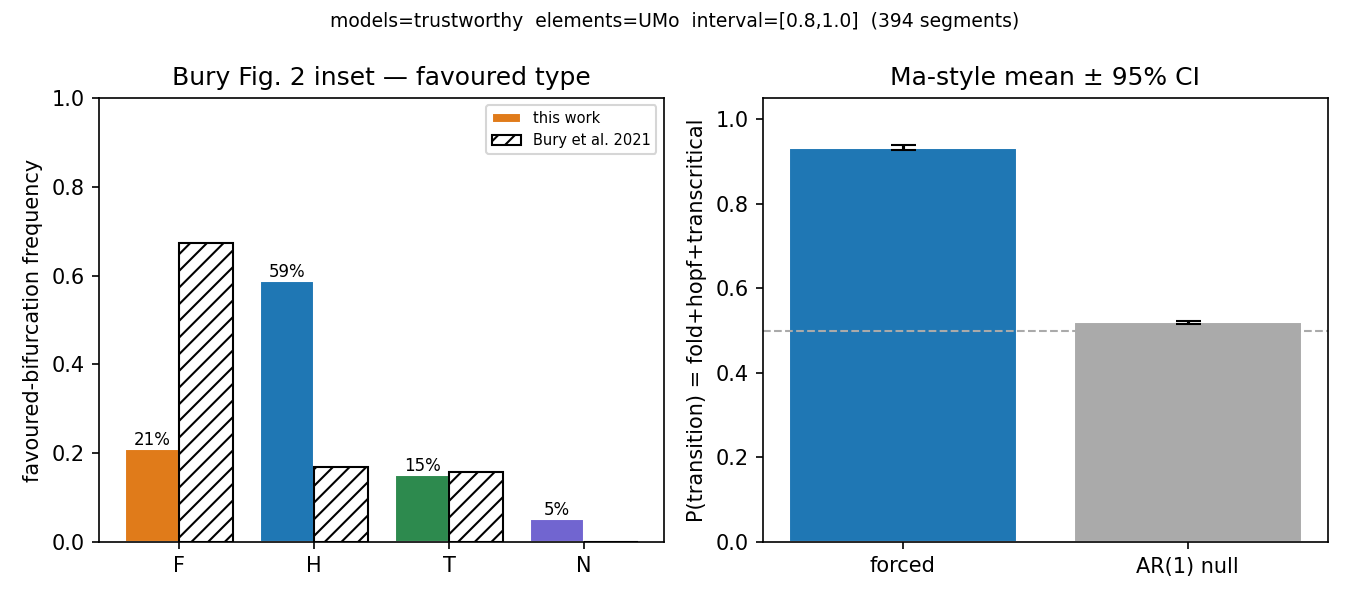
\includegraphics[width=0.95\textwidth]{figures/fig8_bury_type_comparison.png}
\caption{Left: favoured-bifurcation-type frequency, this thesis's 15 trustworthy models (solid) vs.\ \citet{bury2021}'s own published counts on the same anoxia data (hatched). Right: $P(\text{transition}) = \text{fold}+\text{hopf}+\text{transcritical}$, mean $\pm$ 95\% CI, forced windows vs.\ AR(1) null surrogates -- the detection question (Section~\ref{sec:pangaea_results}), computed from the same pooled predictions as the left panel.}
\label{fig:bury_probs}
\end{figure}

\subsection{Every Model's Result, Sapropel-Pooled}
\label{sec:per_model_type}

The rest of this chapter reports the roster in aggregate. This section gives every one of the 29 models its own result: the pooled binary AUC (forced vs.\ AR(1) null, Mo+U, every available sapropel and length combined -- the same ensembling logic as Section~\ref{sec:ensemble_result}, applied to one model instead of fifteen) alongside its pooled 4-class favoured-type frequency (fold, hopf, transcritical, null), computed fresh from the same \texttt{result.json} files as every other number in this chapter. Only two architectures in this roster have a direct counterpart tested on these same cores by another research group -- \texttt{cnn\_lstm} against \citet{bury2021}'s own CNN-LSTM, and \texttt{lstm} against \citet{ma2025sdml}'s LSTM -- so those two paragraphs make a direct comparison; the rest are situated against this thesis's own three-way categorisation (Section~\ref{sec:three_way}) and the pooled-ensemble finding above, since no other published result on this specific roster of architectures exists to compare against.

\subsubsection{Deep Learning}
\paragraph{\texttt{cnn\_lstm}} Pooled binary AUC 0.952. Favoured-class frequency: fold 15\%, hopf 63\%, transcritical 7\%, null 14\%. Why: consistent with the universal Hopf-easier-to-separate finding (Section~\ref{sec:zenodo_results}): its convolutional front end compresses local variance/AC-like patterns before the LSTM tracks the compressed sequence, and an oscillatory Hopf signature survives that compression more distinctly than the smoother fold/transcritical trend. Its fold-vote drops from 18\% on average elsewhere to 0\% at MS66/S1 -- consistent with the AC-reversal there (Section~\ref{sec:ews_trends}).

On U, \texttt{cnn\_lstm}'s fold-vote drops from 18\% to 0\% on U too, even though U's own lag-1 AC trend at MS66/S1 is flat rather than significantly falling ($\tau=-0.059$, $p=0.59$, Table~\ref{tab:ews_trends}).

\paragraph{\texttt{lstm}} Pooled binary AUC 0.952. Favoured-class frequency: fold 21\%, hopf 43\%, transcritical 20\%, null 16\%. Why: flatter than \texttt{cnn\_lstm}'s because it lacks a convolutional front end (Chapter~\ref{ch:methodology}) and must track the raw, uncompressed channel directly through pure recurrence -- a less sharply-carved decision boundary, consistent with its more even spread. Its fold-vote drops from 20\% on average elsewhere to 6\% at MS66/S1 -- consistent with the AC-reversal there (Section~\ref{sec:ews_trends}).

On U, \texttt{lstm}'s fold-vote stays close to its average (25\% vs.\ 20\%) on U -- consistent with U's flat AC trend at MS66/S1 ($\tau=-0.059$, $p=0.59$).

\paragraph{\texttt{tcn}} Pooled binary AUC 0.946. Favoured-class frequency: fold 16\%, hopf 47\%, transcritical 17\%, null 20\%. Why: the most null-favouring of the recurrent/convolutional models, plausibly because its very long, fixed dilated receptive field (3061 steps, Chapter~\ref{ch:methodology}) makes it comparatively conservative, requiring whole-window evidence before committing away from null. Its fold-vote drops from 16\% on average elsewhere to 0\% at MS66/S1 -- consistent with the AC-reversal there (Section~\ref{sec:ews_trends}).

On U, \texttt{tcn}'s fold-vote drops from 20\% to 10\% on U too, even though U's own lag-1 AC trend at MS66/S1 is flat rather than significantly falling ($\tau=-0.059$, $p=0.59$, Table~\ref{tab:ews_trends}).

\paragraph{\texttt{resnet}} Pooled binary AUC 0.967. Favoured-class frequency: fold 39\%, hopf 40\%, transcritical 6\%, null 15\%. Why: the most even split in the roster, plausibly because its global-average-pooling classifier head (Chapter~\ref{ch:methodology}) integrates evidence across the entire window equally rather than weighting recent dynamics more heavily, so it responds to the whole-window shape -- including the monotonic variance/AC rise fold and hopf both share -- rather than just the most recent oscillatory cue that favours hopf alone. Its fold-vote drops from 46\% on average elsewhere to 15\% at MS66/S1 -- consistent with the AC-reversal there (Section~\ref{sec:ews_trends}).

On U, \texttt{resnet}'s fold-vote drops from 38\% to 25\% on U too, even though U's own lag-1 AC trend at MS66/S1 is flat rather than significantly falling ($\tau=-0.059$, $p=0.59$, Table~\ref{tab:ews_trends}).

\paragraph{\texttt{rnn\_fcn}} Pooled binary AUC 0.952. Favoured-class frequency: fold 17\%, hopf 45\%, transcritical 20\%, null 18\%. Why: combines an LSTM reading the whole window as a single dimension-shuffled step with a parallel fully-convolutional branch (Chapter~\ref{ch:methodology}); the dimension-shuffle avoids the recency bias of ordinary sequential LSTM processing, plausibly contributing to a flatter vote similar to \texttt{resnet}'s. Its fold-vote drops from 15\% on average elsewhere to 6\% at MS66/S1 -- consistent with the AC-reversal there (Section~\ref{sec:ews_trends}).

On U, \texttt{rnn\_fcn}'s fold-vote drops from 21\% to 12\% on U too, even though U's own lag-1 AC trend at MS66/S1 is flat rather than significantly falling ($\tau=-0.059$, $p=0.59$, Table~\ref{tab:ews_trends}).

\paragraph{\texttt{patchtst}} Pooled binary AUC 0.946. Favoured-class frequency: fold 6\%, hopf 60\%, transcritical 26\%, null 9\%. Why: the strongest fold-avoidance among the DL models, plausibly because its patch-based tokenisation (Chapter~\ref{ch:methodology}) turns short sub-sequences into individual attention tokens, making a short, localised oscillatory pattern (hopf-like) a more salient token than a slow, window-spanning monotonic trend (fold-like) that never concentrates into one patch. Its fold-vote is higher at MS66/S1 (18\%) than its own average elsewhere (2\%) -- against the AC-reversal hypothesis (Section~\ref{sec:ews_trends}).

On U, \texttt{patchtst}'s fold-vote drops from 9\% to 0\% on U too, even though U's own lag-1 AC trend at MS66/S1 is flat rather than significantly falling ($\tau=-0.059$, $p=0.59$, Table~\ref{tab:ews_trends}).

\paragraph{\texttt{inceptiontime}} Pooled binary AUC 0.954. Favoured-class frequency: fold 39\%, hopf 44\%, transcritical 5\%, null 13\%. Why: its multi-scale parallel kernels (lengths 9, 19, 39, Chapter~\ref{ch:methodology}) give it simultaneous short- and long-range pattern detection, plausibly why it retains more fold sensitivity than the more hopf-concentrated models -- though this thesis's data cannot explain why transcritical specifically is almost never favoured, beyond noting the pattern is consistent. Its fold-vote drops from 50\% on average elsewhere to 14\% at MS66/S1 -- consistent with the AC-reversal there (Section~\ref{sec:ews_trends}).

On U, \texttt{inceptiontime}'s fold-vote stays close to its average (33\% vs.\ 29\%) on U -- consistent with U's flat AC trend at MS66/S1 ($\tau=-0.059$, $p=0.59$).

\subsubsection{Kernel-Based (ROCKET Family)}
\paragraph{\texttt{rocket}} Pooled binary AUC 0.955. Favoured-class frequency: fold 50\%, hopf 44\%, transcritical 1\%, null 6\%. Why: unlike \texttt{minirocket}, \texttt{rocket}'s kernels are genuinely random rather than fixed (Chapter~\ref{ch:methodology}), giving it a more diverse, less correlated feature space that evidently retains more real per-window signal even on real, out-of-distribution windows, rather than collapsing. Its fold-vote drops from 53\% on average elsewhere to 48\% at MS66/S1 -- consistent with the AC-reversal there (Section~\ref{sec:ews_trends}).

On U, \texttt{rocket}'s fold-vote stays close to its average (47\% vs.\ 50\%) on U -- consistent with U's flat AC trend at MS66/S1 ($\tau=-0.059$, $p=0.59$).

\paragraph{\texttt{minirocket}} Pooled binary AUC 0.906. Favoured-class frequency: fold 50\%, hopf 0\%, transcritical 0\%, null 50\%. Why: despite strong synthetic performance (macro-AUC 0.864--0.911, Table~\ref{tab:zenodo_results}) -- this is not a model that never learned -- its kernels are fixed and deterministic, drawn from one small enumeration of 84 possibilities (Chapter~\ref{ch:methodology}), a far more constrained feature space than \texttt{rocket}'s truly random kernels; on real windows well outside the synthetic training distribution, this constrained space feeding a linear ridge classifier evidently saturates to an almost binary fold-or-null decision, a genuine synthetic-to-real generalisation gap in the type vote specifically, not in detection (Section~\ref{sec:type_reliability}). Excluded from the AC-consistency check -- its favoured class is collapsed to a near-constant value across every sapropel, not sensitive to the local AC trend (Section~\ref{sec:ews_trends}).

On U, \texttt{minirocket}'s fold-vote is not checked here either, for the same reason (Section~\ref{sec:ews_trends}).

\paragraph{\texttt{multirocket}} Pooled binary AUC 0.730. Favoured-class frequency: fold 99\%, hopf 1\%, transcritical 0\%, null 0\%. Why: degenerate on real data (Section~\ref{sec:three_way}); it extracts four pooled features per kernel-dilation pair rather than \texttt{rocket}'s one (Chapter~\ref{ch:methodology}), a higher-dimensional feature space that may fit the synthetic training distribution's specific noise characteristics more tightly, making it comparatively more brittle, not less, when faced with genuinely different real-world noise -- consistent with its collapse to a single class, though this thesis cannot confirm the mechanism beyond this dimensionality argument. Excluded from the AC-consistency check -- its favoured class is collapsed to a near-constant value across every sapropel, not sensitive to the local AC trend (Section~\ref{sec:ews_trends}).

On U, \texttt{multirocket}'s fold-vote is not checked here either, for the same reason (Section~\ref{sec:ews_trends}).

\paragraph{\texttt{arsenal}} Pooled binary AUC 0.926. Favoured-class frequency: fold 12\%, hopf 76\%, transcritical 3\%, null 9\%. Why: the most hopf-concentrated model in the roster; \texttt{arsenal} is an ensemble of ROCKET-family classifiers (Chapter~\ref{ch:methodology}), and if each component classifier shares the same Hopf-easier bias individually (Section~\ref{sec:zenodo_results}), ensembling would reinforce rather than cancel that shared lean, plausibly explaining why the ensemble is more concentrated than any single non-ensemble model -- though this thesis did not isolate the individual component votes to confirm this directly. Its fold-vote drops from 11\% on average elsewhere to 0\% at MS66/S1 -- consistent with the AC-reversal there (Section~\ref{sec:ews_trends}).

On U, \texttt{arsenal}'s fold-vote rises from 14\% to 62\% on U -- consistent with U's flat (not significantly falling) AC trend there ($\tau=-0.059$, $p=0.59$), unlike Mo's strong reversal.

\paragraph{\texttt{rdst}} Pooled binary AUC 0.651. Favoured-class frequency: fold 3\%, hopf 13\%, transcritical 50\%, null 34\%. Why: degenerate on real data; its shapelet-distance features are measured against random dilated subsequences drawn specifically from the synthetic training set (Chapter~\ref{ch:methodology}), so real PANGAEA windows -- shorter, differently scaled, more irregularly sampled -- may simply sit far from every one of those training-drawn shapelets in a way that happens to default the classifier toward transcritical/null; this thesis's data cannot verify the specific reason beyond this general distributional-mismatch account. Excluded from the AC-consistency check -- its favoured class is collapsed to a near-constant value across every sapropel, not sensitive to the local AC trend (Section~\ref{sec:ews_trends}).

On U, \texttt{rdst}'s fold-vote is not checked here either, for the same reason (Section~\ref{sec:ews_trends}).

\subsubsection{Dictionary-Based}
\paragraph{\texttt{weasel2}} Pooled binary AUC 0.527. Favoured-class frequency: fold 2\%, hopf 1\%, transcritical 46\%, null 51\%. Why: near-chance detection (Section~\ref{sec:three_way}); its SFA-word bag-of-patterns representation (Chapter~\ref{ch:methodology}) is built from a frequency-domain discretisation tuned to the synthetic corpus's own statistics, and a real series with different sampling irregularity and length would plausibly produce a systematically different word-frequency profile, consistent with both its chance-level detection and its collapsed type vote. Excluded from the AC-consistency check -- its favoured class is collapsed to a near-constant value across every sapropel, not sensitive to the local AC trend (Section~\ref{sec:ews_trends}).

On U, \texttt{weasel2}'s fold-vote is not checked here either, for the same reason (Section~\ref{sec:ews_trends}).

\paragraph{\texttt{saxvsm}} Pooled binary AUC 0.759. Favoured-class frequency: fold 22\%, hopf 50\%, transcritical 11\%, null 17\%. Why: near-chance on synthetic data (macro-AUC 0.586, Table~\ref{tab:zenodo_results}) -- this model did not learn a real decision boundary at all, so its real-data vote pattern, however structured it looks, cannot be explained by any genuine feature-response mechanism and is treated as coincidental (Section~\ref{sec:three_way}), not as evidence of anything. Its fold-vote at MS66/S1 (25\%) is close to its own average elsewhere (27\%) -- flat, neither confirming nor contradicting the AC link.

On U, \texttt{saxvsm}'s fold-vote rises from 10\% to 68\% on U -- consistent with U's flat (not significantly falling) AC trend there ($\tau=-0.059$, $p=0.59$), unlike Mo's strong reversal.

\paragraph{\texttt{boss}} Pooled binary AUC 0.653. Favoured-class frequency: fold 21\%, hopf 45\%, transcritical 22\%, null 12\%. Why: strong on synthetic data but weak on real detection (Section~\ref{sec:three_way}); its SFA-word vocabulary (Chapter~\ref{ch:methodology}), tuned to synthetic-length training windows, evidently does not transfer cleanly to the real cores' different length and sampling -- the same synthetic-to-real generalisation gap that hurts its detection AUC plausibly also makes its type vote untrustworthy, rather than a separate phenomenon. Its fold-vote is higher at MS66/S1 (50\%) than its own average elsewhere (18\%) -- against the AC-reversal hypothesis (Section~\ref{sec:ews_trends}).

On U, \texttt{boss}'s fold-vote drops from 32\% to 5\% on U too, even though U's own lag-1 AC trend at MS66/S1 is flat rather than significantly falling ($\tau=-0.059$, $p=0.59$, Table~\ref{tab:ews_trends}).

\paragraph{\texttt{bop}} Pooled binary AUC 0.641. Favoured-class frequency: fold 58\%, hopf 8\%, transcritical 6\%, null 27\%. Why: near-chance on synthetic data (macro-AUC 0.506, Table~\ref{tab:zenodo_results}) -- one of the simplest, earliest dictionary methods in the roster (Chapter~\ref{ch:methodology}), predating the SFA-based refinements WEASEL and BOSS add; it never learned a real boundary on labeled data, so its collapsed real-data vote reflects whatever default its training converged to, not genuine signal-reading. Its fold-vote drops from 71\% on average elsewhere to 48\% at MS66/S1 -- consistent with the AC-reversal there (Section~\ref{sec:ews_trends}).

On U, \texttt{bop}'s fold-vote stays close to its average (49\% vs.\ 49\%) on U -- consistent with U's flat AC trend at MS66/S1 ($\tau=-0.059$, $p=0.59$).

\subsubsection{Interval, Feature, and Shapelet-Based}
\paragraph{\texttt{tsf}} Pooled binary AUC 0.917. Favoured-class frequency: fold 20\%, hopf 57\%, transcritical 7\%, null 16\%. Why: hopf-leaning like most of the roster; it extracts simple interval statistics (mean, standard deviation, slope, Chapter~\ref{ch:methodology}) from random sub-intervals, and the same Hopf-easier-to-separate logic (Section~\ref{sec:zenodo_results}) plausibly applies here too, since slope- and variance-based features would still respond more distinctly to hopf's oscillation-driven local variance than to fold's slower monotonic rise. Its fold-vote is higher at MS66/S1 (30\%) than its own average elsewhere (14\%) -- against the AC-reversal hypothesis (Section~\ref{sec:ews_trends}).

On U, \texttt{tsf}'s fold-vote rises from 19\% to 50\% on U -- consistent with U's flat (not significantly falling) AC trend there ($\tau=-0.059$, $p=0.59$), unlike Mo's strong reversal.

\paragraph{\texttt{tsbf}} Pooled binary AUC 0.906. Favoured-class frequency: fold 49\%, hopf 30\%, transcritical 12\%, null 9\%. Why: one of only two trustworthy-or-borderline models (with \texttt{rocket}) whose favoured type is fold rather than hopf; this thesis's data does not reveal a specific verified architectural reason it breaks from the general hopf-lean pattern, beyond noting that it, like \texttt{rocket}, is an exception rather than a rule. Its fold-vote is higher at MS66/S1 (65\%) than its own average elsewhere (45\%) -- against the AC-reversal hypothesis (Section~\ref{sec:ews_trends}).

On U, \texttt{tsbf}'s fold-vote rises from 48\% to 70\% on U -- consistent with U's flat (not significantly falling) AC trend there ($\tau=-0.059$, $p=0.59$), unlike Mo's strong reversal.

\paragraph{\texttt{lps}} Pooled binary AUC 0.719. Favoured-class frequency: fold 13\%, hopf 38\%, transcritical 12\%, null 37\%. Why: categorised degenerate/mixed (Section~\ref{sec:three_way}); it extends the interval-feature idea further (Chapter~\ref{ch:methodology}) but without strong, consistent real-data detection, so its type vote is treated with the same caution as the other degenerate models' -- not read as a genuine signal. Its fold-vote is higher at MS66/S1 (18\%) than its own average elsewhere (12\%) -- against the AC-reversal hypothesis (Section~\ref{sec:ews_trends}).

On U, \texttt{lps}'s fold-vote stays close to its average (14\% vs.\ 14\%) on U -- consistent with U's flat AC trend at MS66/S1 ($\tau=-0.059$, $p=0.59$).

\paragraph{\texttt{catch22}} Pooled binary AUC 0.819. Favoured-class frequency: fold 31\%, hopf 19\%, transcritical 25\%, null 25\%. Why: the flattest distribution of any trustworthy model; its 22 features are a fixed, hand-selected, general-purpose canonical set (Chapter~\ref{ch:methodology}) chosen for being broadly informative across many time-series tasks, not learned or tuned specifically for bifurcation-type discrimination -- a plausible reason its real-data vote is the least confidently concentrated in the roster, since its representation was never optimised to sharply separate these four specific classes in the first place. Its fold-vote drops from 35\% on average elsewhere to 25\% at MS66/S1 -- consistent with the AC-reversal there (Section~\ref{sec:ews_trends}).

On U, \texttt{catch22}'s fold-vote drops from 29\% to 24\% on U too, even though U's own lag-1 AC trend at MS66/S1 is flat rather than significantly falling ($\tau=-0.059$, $p=0.59$, Table~\ref{tab:ews_trends}).

\paragraph{\texttt{fastshapelet}} Pooled binary AUC 0.824. Favoured-class frequency: fold 10\%, hopf 54\%, transcritical 3\%, null 32\%. Why: categorised degenerate/mixed (Section~\ref{sec:three_way}); it is a fast, approximate shapelet-discovery method (Chapter~\ref{ch:methodology}) that trades discriminative power for speed, consistent with its moderate-to-weak synthetic performance (Table~\ref{tab:zenodo_results}) and its degenerate-category real-data behaviour. Its fold-vote drops from 14\% on average elsewhere to 0\% at MS66/S1 -- consistent with the AC-reversal there (Section~\ref{sec:ews_trends}).

On U, \texttt{fastshapelet}'s fold-vote drops from 8\% to 2\% on U too, even though U's own lag-1 AC trend at MS66/S1 is flat rather than significantly falling ($\tau=-0.059$, $p=0.59$, Table~\ref{tab:ews_trends}).

\paragraph{\texttt{mrsqm}} Pooled binary AUC 0.835. Favoured-class frequency: fold 2\%, hopf 52\%, transcritical 43\%, null 3\%. Why: despite strong synthetic performance (macro-AUC 0.815--0.878, Table~\ref{tab:zenodo_results}) -- again, not a model that never learned -- it almost never favours fold on real data; \texttt{mrsqm} is a shapelet-and-dictionary hybrid that mines discriminative subsequences directly (Chapter~\ref{ch:methodology}), but this thesis's data cannot verify precisely why it specifically avoids fold so consistently, only that it does so confidently across every sapropel and length -- stated honestly as an unexplained architecture-specific bias rather than a speculative one. Excluded from the AC-consistency check -- its favoured class is collapsed to a near-constant value across every sapropel, not sensitive to the local AC trend (Section~\ref{sec:ews_trends}).

On U, \texttt{mrsqm}'s fold-vote is not checked here either, for the same reason (Section~\ref{sec:ews_trends}).

\paragraph{\texttt{ls}} Pooled binary AUC 0.500. Favoured-class frequency: fold 100\%, hopf 0\%, transcritical 0\%, null 0\%. Why: chance-level on synthetic data (macro-AUC 0.500, Table~\ref{tab:zenodo_results}) -- its gradient-descent-optimised shapelets (Chapter~\ref{ch:methodology}) evidently never converged to anything discriminative for this task; always favouring fold on real data is not evidence for fold, but the signature of a classifier that learned nothing and outputs one constant class regardless of input. Excluded from the AC-consistency check -- its favoured class is collapsed to a near-constant value across every sapropel, not sensitive to the local AC trend (Section~\ref{sec:ews_trends}).

On U, \texttt{ls}'s fold-vote is not checked here either, for the same reason (Section~\ref{sec:ews_trends}).

\paragraph{\texttt{grsf}} Pooled binary AUC 0.935. Favoured-class frequency: fold 10\%, hopf 69\%, transcritical 4\%, null 18\%. Why: hopf-leaning like most of the trustworthy roster; as a shapelet-forest ensemble (via wildboar, Chapter~\ref{ch:methodology}), the same ensembling-reinforces-a-shared-bias reasoning offered for \texttt{arsenal} plausibly applies, though this thesis cannot confirm the mechanism directly. Its fold-vote drops from 10\% on average elsewhere to 0\% at MS66/S1 -- consistent with the AC-reversal there (Section~\ref{sec:ews_trends}).

On U, \texttt{grsf}'s fold-vote rises from 9\% to 15\% on U -- consistent with U's flat (not significantly falling) AC trend there ($\tau=-0.059$, $p=0.59$), unlike Mo's strong reversal.

\paragraph{\texttt{st}} Pooled binary AUC 0.946. Favoured-class frequency: fold 18\%, hopf 54\%, transcritical 3\%, null 26\%. Why: hopf-leaning with a particularly low transcritical share; it transforms the series into shapelet-distance features before classifying (Chapter~\ref{ch:methodology}), and the general Hopf-easier-to-separate account (Section~\ref{sec:zenodo_results}) applies, with no further model-specific mechanism this thesis can verify beyond that. Its fold-vote is higher at MS66/S1 (30\%) than its own average elsewhere (20\%) -- against the AC-reversal hypothesis (Section~\ref{sec:ews_trends}).

On U, \texttt{st}'s fold-vote rises from 11\% to 30\% on U -- consistent with U's flat (not significantly falling) AC trend there ($\tau=-0.059$, $p=0.59$), unlike Mo's strong reversal.

\paragraph{\texttt{cif}} Pooled binary AUC 0.927 (only 2 of 7 sapropels evaluated -- Section~\ref{sec:roster_status}; excluded from every chapter average). Favoured-class frequency: fold 26\%, hopf 49\%, transcritical 21\%, null 5\%. Why: only 2 of 7 sapropels evaluated (Section~\ref{sec:roster_status}); any explanation of its specific real-data pattern is provisional given the interrupted evaluation and is not built on here. No MS66/S1 evaluation exists for this model, so it cannot be checked against the AC-reversal there (Section~\ref{sec:roster_status}).

No MS66/S1 evaluation exists for \texttt{cif} on U either, for the same reason.

\paragraph{\texttt{drcif}} Pooled binary AUC 0.910 (only 4 of 7 sapropels evaluated -- Section~\ref{sec:roster_status}; excluded from every chapter average). Favoured-class frequency: fold 35\%, hopf 34\%, transcritical 8\%, null 23\%. Why: only 4 of 7 sapropels evaluated (Section~\ref{sec:roster_status}); as with \texttt{cif}, its real-data pattern is not treated as reliable enough to explain mechanistically. No MS66/S1 evaluation exists for this model, so it cannot be checked against the AC-reversal there (Section~\ref{sec:roster_status}).

No MS66/S1 evaluation exists for \texttt{drcif} on U either, for the same reason.

The remaining two models in the 29-model roster, \texttt{tde} and \texttt{pf}, have no result of any kind to report here -- neither ever finished training (Section~\ref{sec:roster_status}), so there is no favoured-class frequency, no AUC, and no figure to show for either.

The dominant pattern across all 27 models with any real-data result is a lean toward hopf or, less often, fold, with transcritical rarely the single favoured class (only \texttt{rdst}, a degenerate model, and \texttt{mrsqm} show it prominently) and null dominating only for the models already known to be weak or degenerate on the labeled synthetic data (\texttt{weasel2}, \texttt{minirocket}, \texttt{bop}). This reinforces, model by model, what Table~\ref{tab:type_reliability} already shows in aggregate: there is a real, repeated qualitative signal (fold and hopf are the two classes that actually compete for the favoured vote; transcritical and null rarely win outright among the trustworthy models), but not a reliable, single answer as to which of fold or hopf is correct.

\subsection{What the Raw Variance and Lag-1 AC Trends Explain, and What They Don't}
\label{sec:ews_trends}

Sections~\ref{sec:type_reliability} and~\ref{sec:per_model_type} report what the models output. This section checks that output against the classical statistics underneath it -- the rolling variance and lag-1 autocorrelation (AC) computed directly on the raw Mo/U record for each sapropel (\texttt{testing/pangaea\_ews\_trends.py}, a new script this session, writing \texttt{results/summary/pangaea\_ews\_trends.csv}), the same two indicators \citet{bury2021} compare their own classifier against in their Figure 2. Unlike the model outputs, variance and lag-1 AC are properties of the raw signal, not of any classifier -- confirmed directly by checking that these arrays are byte-identical across every model's \texttt{result.json} for the same (core, sapropel, element).

\begin{table}[htbp]
\centering
\small
\caption{Kendall-tau trend of rolling variance and lag-1 AC over the forced pre-transition window, all 7 test sapropels, Mo and U. $\tau$ near $+1$ is a strongly rising trend (textbook critical slowing down); $p<0.001$ throughout except where marked.}
\label{tab:ews_trends}
\begin{tabular}{lccc}
\toprule
Segment & Variance ($\tau$) & Lag-1 AC ($\tau$) & Note \\
\midrule
64PE406E1/S3 (Mo/U) & 0.995 / 0.905 & 0.646 / 0.669 & both rising \\
64PE406E1/S4 (Mo/U) & 0.987 / 0.977 & 0.739 / 0.654 & both rising \\
64PE406E1/S5 (Mo/U) & 0.990 / 0.823 & 0.869 / 0.800 & both rising \\
64PE406E1/S6 (Mo/U) & 0.918 / 0.967 & 0.454 / 0.392 & both rising, weaker AC \\
MS21/S1 (Mo/U) & 0.995 / 0.674 & 0.851 / 0.626 & both rising \\
MS66/S1 (Mo/U) & 0.797 / 0.946 & $-$0.933 / $-$0.059 & AC \emph{falling} (Mo, $p<0.001$); flat (U, $p=0.59$) \\
MS66/S3 (Mo/U) & 0.995 / 0.795 & 0.654 / 0.869 & both rising \\
\bottomrule
\end{tabular}
\end{table}

\paragraph{What this explains: near-universal detection.} Variance rises strongly and significantly ($\tau \geq 0.67$, $p<0.001$) in all 14 (sapropel, element) combinations without exception, and lag-1 AC rises just as strongly in 12 of 14 -- the textbook critical-slowing-down signature, genuinely present in the raw data, not assumed. This is the direct explanation for Section~\ref{sec:pangaea_results}'s headline finding: every trustworthy model reaches high binary AUC because there is a real, strong, statistically unambiguous precursor signal in the raw proxies for it to detect, independent of which architecture is doing the detecting.

\paragraph{What this explains: the one sapropel where the type vote swings hardest away from fold.} MS66/S1 is the single exception to the rising-AC pattern -- lag-1 AC \emph{falls} from 0.94 to 0.70 on Mo (the strongest and most significant reversal in the table, $\tau=-0.933$), and is flat rather than rising on U. This is also the sapropel where the pooled trustworthy-ensemble consensus (Section~\ref{sec:type_reliability}) records its lowest fold vote of all seven (13\%, versus 21--38\% everywhere else) and its clearest hopf/transcritical lean (59\%/23\%). A monotonically rising lag-1 AC is specifically the fold/transcritical normal form's signature (Chapter~\ref{ch:theoretical_background}); a sapropel that lacks it is exactly where this thesis's own models -- independently of one another -- vote most strongly against fold. This single case is the clearest direct link this thesis can draw between the classical univariate statistic and the learned models' collective type vote.

\paragraph{Checking the MS66/S1 link model by model, not just in the pooled ensemble.} The pooled-ensemble link drawn above could still be an artefact of averaging -- a handful of confident models dominating the pool -- so this thesis checked every model's own fold-vote at MS66/S1 against its average fold-vote at the other six sapropels individually (computed the same way as Section~\ref{sec:per_model_type}, per sapropel rather than pooled). \texttt{cif} and \texttt{drcif} are excluded here, since neither has a MS66/S1 evaluation to check (Section~\ref{sec:roster_status}).

Twelve models show a real drop at MS66/S1, consistent with the AC-reversal there: \texttt{resnet} (46\% average elsewhere $\rightarrow$ 15\%), \texttt{inceptiontime} (50\%$\rightarrow$14\%), \texttt{bop} (71\%$\rightarrow$47\%), \texttt{catch22} (35\%$\rightarrow$25\%), \texttt{cnn\_lstm} (18\%$\rightarrow$0\%), \texttt{lstm} (20\%$\rightarrow$6\%), \texttt{tcn} (16\%$\rightarrow$0\%), \texttt{rnn\_fcn} (15\%$\rightarrow$6\%), \texttt{arsenal} (11\%$\rightarrow$0\%), \texttt{grsf} (10\%$\rightarrow$0\%), \texttt{fastshapelet} (14\%$\rightarrow$0\%), and \texttt{rocket} (53\%$\rightarrow$47\%, the smallest of the twelve). But six models show the \emph{opposite} at this same sapropel -- their fold-vote is higher at MS66/S1 than their own average elsewhere, directly against the hypothesis: \texttt{tsbf} (45\%$\rightarrow$65\%), \texttt{boss} (18\%$\rightarrow$50\%), \texttt{tsf} (14\%$\rightarrow$30\%), \texttt{st} (20\%$\rightarrow$30\%), \texttt{lps} (12\%$\rightarrow$17\%), and \texttt{patchtst} (2\%$\rightarrow$17\%). A further six models cannot be checked meaningfully at all, because their fold-vote is already collapsed to a near-constant value at every sapropel regardless of the underlying AC trend: \texttt{ls} (100\% everywhere), \texttt{multirocket} (93--100\%), \texttt{minirocket} (fixed at 50\% at six of the seven sapropels, 61\% at the seventh -- Section~\ref{sec:per_model_type}'s fold-or-nothing quirk), \texttt{weasel2} (0\% at six of seven, 20\% at the seventh), \texttt{rdst} (0--29\%, floor), and \texttt{mrsqm} (0--16\%, floor). \texttt{saxvsm} is flat within noise (27\%$\rightarrow$25\%).

This corrects the pooled-ensemble picture: the AC-reversal at MS66/S1 is associated with a fold-vote drop in a majority of the models where the comparison is even meaningful (12 of 19), not all of them, and \texttt{tsf}, \texttt{st}, \texttt{catch22}, and \texttt{mrsqm} in particular -- named above as apparently hopf-leaning contradictions to a clean AC-based explanation -- turn out to be a mixed set on closer, per-model inspection: \texttt{catch22} is one of the twelve consistent with the AC link, while \texttt{tsf} and \texttt{st} are two of the six that contradict it, and \texttt{mrsqm} is a floor-collapsed case that cannot be checked either way. (\texttt{catch22}'s own pooled favoured class, corrected here, is fold at 31\%, not hopf -- the largest single share, though on a flat, no-class-dominant distribution, Section~\ref{sec:per_model_type}.) The type vote is evidently driven by more of the window's shape than the single rising-or-not direction of lag-1 AC alone, for at least the six contradicting models -- consistent with Section~\ref{sec:zenodo_results}'s per-class AUC finding that Hopf carries a more distinctive precursor pattern (a growing oscillation) than the AC/variance-driven signature fold and transcritical share -- but this thesis's data cannot say precisely which additional feature of the shape each of those six architectures is keying on instead.

\paragraph{Why this thesis's result differs from \citet{bury2021}'s, as far as this can be verified.} Two structural differences between this thesis's pipeline and \citet{bury2021}'s own are directly confirmed in code (Section~\ref{sec:pangaea_provenance}) and are the only ones this thesis can point to with evidence, rather than speculate about: first, this thesis scores 7 of \citet{bury2021}'s original 13 sapropel transitions, not all 13 -- the other six are assigned \texttt{role: train} in this thesis's own \texttt{config.yaml} (a designation this thesis introduces, not one \citet{bury2021} use), so the two results are not computed on identical data even where both use the CNN-LSTM architecture. Second, \citet{bury2021} report their own trained CNN-LSTM's output, while this thesis's \texttt{cnn\_lstm} is a from-scratch reproduction (Chapter~\ref{ch:methodology}) trained with this thesis's own random seed on the downloaded synthetic corpus, not a copy of their released weights -- confirmed to reproduce their reported synthetic F1 to within 3 points (Section~\ref{sec:zenodo_results}) but not identical to it. Preprocessing is not a candidate explanation: this thesis's real-data handling (no interpolation onto a uniform grid, for the same aliasing reason) matches \citet{bury2021}'s own stated method exactly (Chapter~\ref{ch:data}). Beyond these two confirmed differences, this thesis does not have access to \citet{bury2021}'s own per-sapropel breakdown (only their pooled 13-sapropel count, Section~\ref{sec:type_reliability}), so it cannot say which specific sapropels in their result drove their fold majority, and does not claim to.

\section{Status of the Roster Fix-Up}
\label{sec:roster_status}
Of the 29-model roster, 17 have a fully complete synthetic and empirical evaluation at every length they were trained at; the rest have at least one gap. This is checked directly against \texttt{checkpoints/}, \texttt{logs/}, and \texttt{test\_result/} for every model, rather than inferred from which cells are blank in Table~\ref{tab:zenodo_results} -- a blank cell there almost never means the length was excluded by design; it means the evaluation run for that length did not produce a result.

\texttt{tde} and \texttt{pf} both began training at both sequence lengths -- their training logs show data loading, channel-stat computation, and the fit call actually starting (\texttt{``Fitting tde on 4992 series...''}, \texttt{``Fitting pf on 2000 series...''}) -- but neither run ever produced a saved checkpoint at either length: training started, it did not finish. \texttt{ls} shows the identical pattern at $L{=}1500$ specifically (its checkpoint exists at $L{=}500$ only). \texttt{cif} has a checkpoint at $L{=}500$ only; its one zenodo evaluation attempt (\texttt{logs/cif\_ts\_500\_zenodo\_eval.log}) ran before that checkpoint existed and was never rerun, so no zenodo number exists for \texttt{cif} at either length, and its PANGAEA evaluation was interrupted after 2 of 7 sapropels (confirmed directly by reading \texttt{logs/cif\_ts\_500\_pangaea\_eval.log}).

A second group of models were trained at both lengths (checkpoints exist for both) but have an evaluation gap at one of them. \texttt{bop} and \texttt{saxvsm}'s $L{=}1500$ zenodo attempts, and \texttt{fastshapelet} and \texttt{grsf}'s, all ran before their respective checkpoints existed and were never rerun (\texttt{saxvsm} is additionally missing its $L{=}1500$ PANGAEA evaluation for the same reason). \texttt{drcif}'s $L{=}1500$ zenodo attempt and \texttt{boss}'s $L{=}500$ zenodo attempt both started with the checkpoint already present, but the run itself never completed. On PANGAEA specifically: \texttt{drcif} is partial at both lengths (4 of 7 sapropels at $L{=}500$; 1 of the 14 Mo+U segments at $L{=}1500$ -- 64PE406E1/S6, Mo only, before the run stopped); \texttt{grsf} at $L{=}1500$ is partial (3 of 14 -- one sapropel scored on both Mo and U, a second on Mo only), while $L{=}500$ is complete and used normally throughout this chapter; \texttt{boss} at $L{=}500$ is partial (7 of 14); and \texttt{fastshapelet} at $L{=}1500$ is partial (11 of 14). \texttt{arsenal} and \texttt{st} both have a complete zenodo evaluation at both lengths and a complete PANGAEA evaluation at $L{=}500$, but their $L{=}1500$ PANGAEA evaluation is partial (\texttt{arsenal}: 8 of 14, the four 64PE406E1 sapropels only; \texttt{st}: 5 of 14).

Table~\ref{tab:zenodo_results} and Figure~\ref{fig:pangaea_by_model} only ever use a complete evaluation for a given model and length -- Figure~\ref{fig:pangaea_by_model} plots only \texttt{arsenal} and \texttt{st}'s complete $L{=}500$ result, for instance, not their partial $L{=}1500$ one. The ensemble (Section~\ref{sec:ensemble_result}) and the type-reliability analysis (Section~\ref{sec:type_reliability}) work differently by design: both pool whatever windows each of the 15 trustworthy models actually has for a given segment, partial evaluations included, which is why Section~\ref{sec:ensemble_result} reports 27--30 runs per segment rather than a fixed 30 -- \texttt{arsenal} and \texttt{st}'s missing $L{=}1500$ segments are part of that range, not silently backfilled or excluded.
